%%%%%%%%%%%%%%%%%%%%%%%%%%%%%%%%%%%%%%%%%
% Short Sectioned Assignment
% LaTeX Template
% Version 1.0 (5/5/12)
%
% This template has been downloaded from:
% http://www.LaTeXTemplates.com
%
% Original author:
% Frits Wenneker (http://www.howtotex.com)
%
% License:
% CC BY-NC-SA 3.0 (http://creativecommons.org/licenses/by-nc-sa/3.0/)
%
%%%%%%%%%%%%%%%%%%%%%%%%%%%%%%%%%%%%%%%%%

%----------------------------------------------------------------------------------------
%	PACKAGES AND OTHER DOCUMENT CONFIGURATIONS
%----------------------------------------------------------------------------------------

\documentclass[paper=a4, fontsize=11pt]{scrartcl} % A4 paper and 11pt font size

\usepackage[T1]{fontenc} % Use 8-bit encoding that has 256 glyphs
\usepackage{fourier} % Use the Adobe Utopia font for the document - comment this line to return to the LaTeX default
\usepackage[english]{babel} % English language/hyphenation
\usepackage{amsmath,amsfonts,amsthm} % Math packages

\usepackage{lipsum} % Used for inserting dummy 'Lorem ipsum' text into the template
\usepackage{graphicx}

\usepackage{sectsty} % Allows customizing section commands
\allsectionsfont{\centering \normalfont\scshape} % Make all sections centered, the default font and small caps

\usepackage{fancyhdr} % Custom headers and footers
\pagestyle{fancyplain} % Makes all pages in the document conform to the custom headers and footers
\fancyhead{} % No page header - if you want one, create it in the same way as the footers below
\fancyfoot[L]{} % Empty left footer
\fancyfoot[C]{} % Empty center footer
\fancyfoot[R]{\thepage} % Page numbering for right footer
\renewcommand{\headrulewidth}{0pt} % Remove header underlines
\renewcommand{\footrulewidth}{0pt} % Remove footer underlines
\setlength{\headheight}{13.6pt} % Customize the height of the header

\numberwithin{equation}{section} % Number equations within sections (i.e. 1.1, 1.2, 2.1, 2.2 instead of 1, 2, 3, 4)
\numberwithin{figure}{section} % Number figures within sections (i.e. 1.1, 1.2, 2.1, 2.2 instead of 1, 2, 3, 4)
\numberwithin{table}{section} % Number tables within sections (i.e. 1.1, 1.2, 2.1, 2.2 instead of 1, 2, 3, 4)

\setlength\parindent{0pt} % Removes all indentation from paragraphs - comment this line for an assignment with lots of text

%----------------------------------------------------------------------------------------
%	TITLE SECTION
%----------------------------------------------------------------------------------------

\newcommand{\horrule}[1]{\rule{\linewidth}{#1}} % Create horizontal rule command with 1 argument of height

\title{	
\normalfont \normalsize 
\textsc{University of Iowa, Professor Omar Haider} \\ [25pt] % Your university, school and/or department name(s)
\horrule{0.5pt} \\[0.4cm] % Thin top horizontal rule
\huge Databases in OpenEMR \\ % The assignment title
\horrule{2pt} \\[0.5cm] % Thick bottom horizontal rule
}

\author{Junhyuk Kang} % Your name

\date{Sep 13, 2016 ~ Sep 19, 2016 } % Today's date or a custom date


\begin{document}

\maketitle % Print the title

%----------------------------------------------------------------------------------------
%	PROBLEM 1
%----------------------------------------------------------------------------------------

\section{Assignments}

\begin{enumerate}
  \item Where are the patients data stored? It is likely to be in a MySQL database
  \item Where is the location of the database
  \item Schema of the database(Tables, column's of each table
  \item User-name, Password for the database
  \item Install MySQL administrator
\end{enumerate}




%----------------------------------------------------------------------------------------
%	PROBLEM 2
%----------------------------------------------------------------------------------------

\section{Answer Steps}

%------------------------------------------------
\begin{itemize}
	\item Started with Db.opt, nothing was in this file
	\item Opened $Patient_data.frm,patient_data.MYI$ with txt, but could not read
	\item Opened files with subrime text, and found over 60 lines of encrypted keys
		\graphicspath {{C:/pictures/}}
		\begin{itemize}
		\item
		 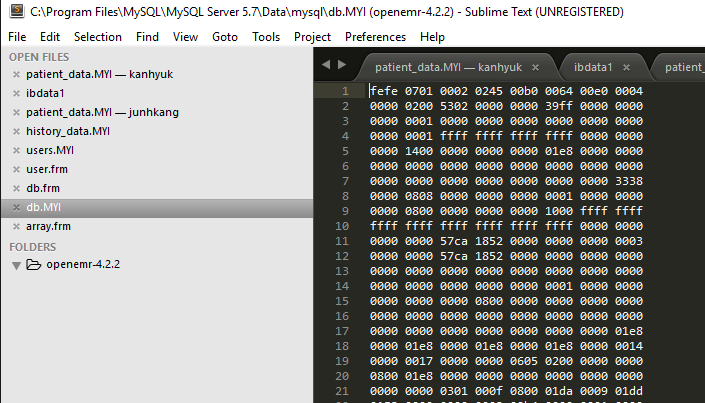
\includegraphics[width = 15cm, height=8cm]{dataaskey.png}
		\end{itemize}
\vspace{2cm}
	\item On localhost/openemr, under patient reminders/Log tab, we can find every log
		\begin{itemize}
		\item
		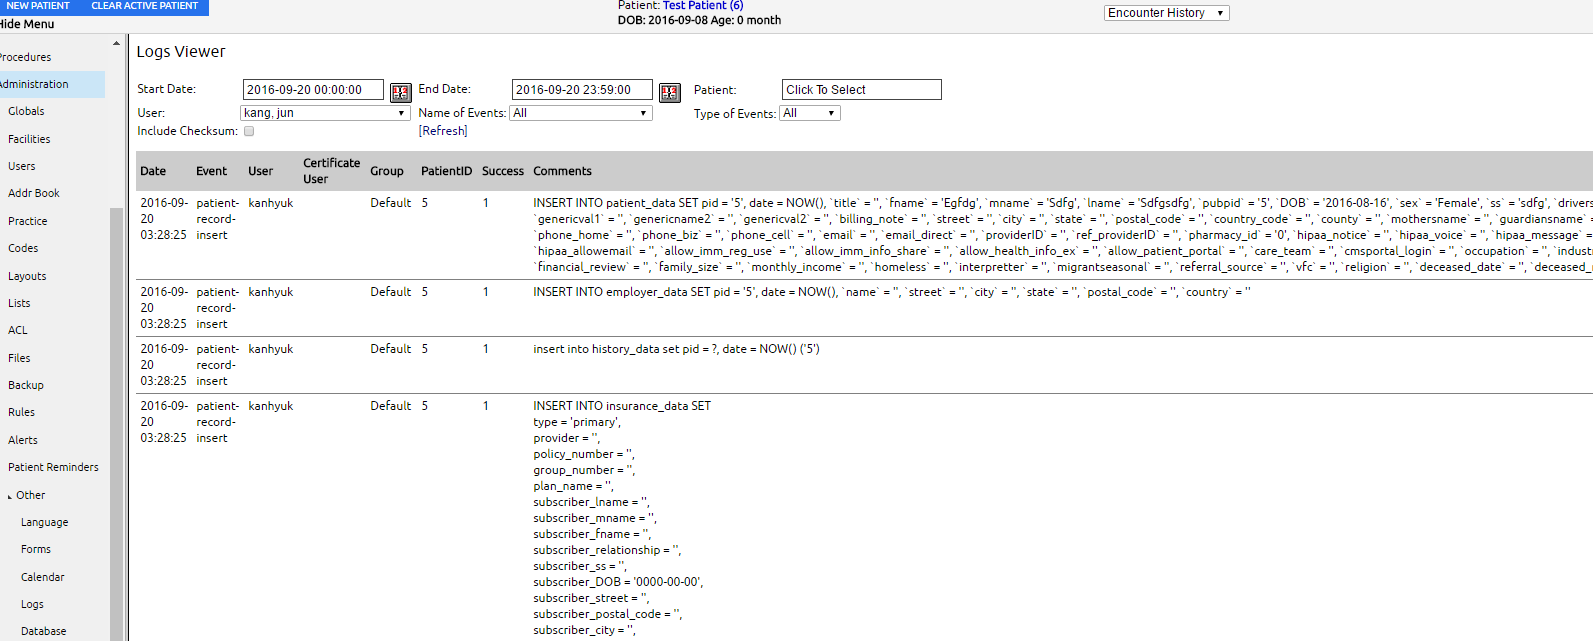
\includegraphics[width = 15cm, height=8cm]{1stlog.jpg}
		\end{itemize}
\vspace{2cm}
	\item To find where is username, password data stored
		\begin{itemize}
		\item Add new user under Administration tab
			\begin{itemize}
			\item
			 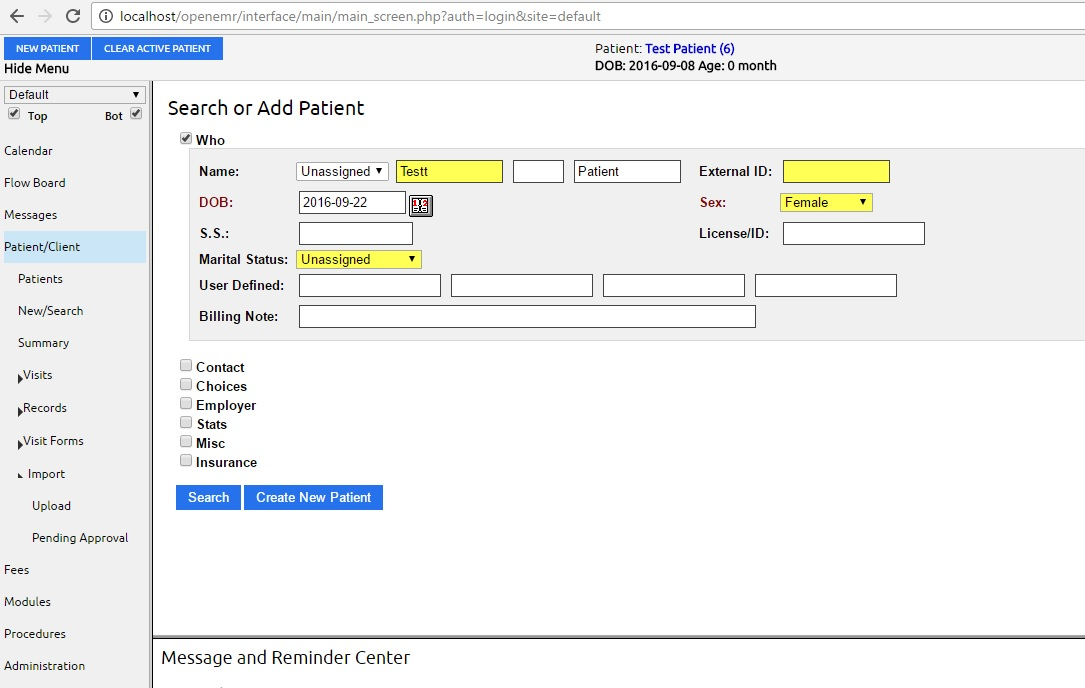
\includegraphics[width = 15cm, height=8cm]{creatingnewpatient.jpg}
		\end{itemize}
		\item Give different access control
			\begin{itemize}
				\item Accounting
				\item Front Office
				\item Clinician
					\begin{itemize}
						\item
						 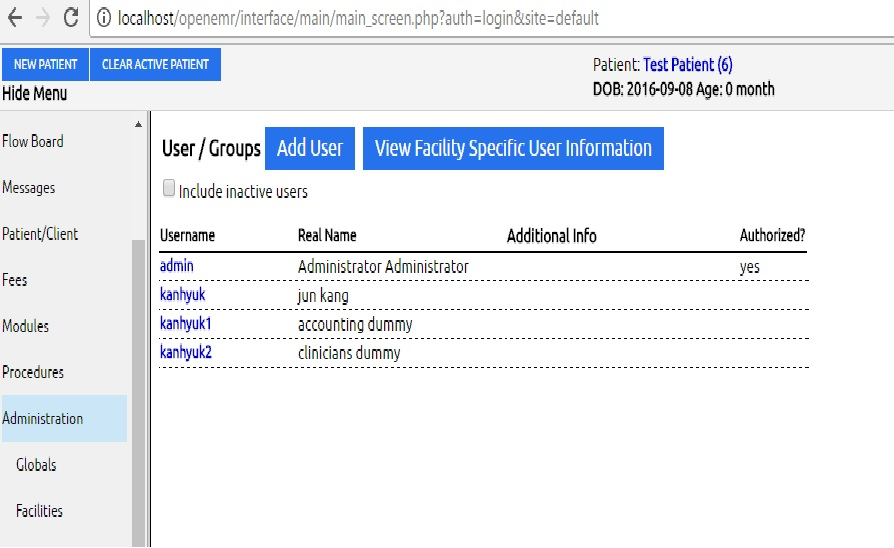
\includegraphics[width = 15cm, height=8cm]{varioususers.jpg}
					\end{itemize}
			\end{itemize}
		
		\item Tried to find any new fille added after adding new account, but there was no change
		\item Found changes in keys in datafile
			\begin{itemize}
				\item Changes in line 8~9 in $Patient_data.MYI$
				\item from 0000 19a0 0000 0832 0000 0000 0000 0002 0000 0000
				\item to     0000 1924 0000 0000 0000 0000 0000 0000 ffff ffff
			\end{itemize}
\end{itemize}

\vspace{2cm}
		\item Logged in MySQL workbench
		\item Found 'database' under schemas
		\begin{itemize}
			\item
			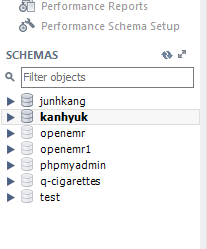
\includegraphics[width = 5cm, height=3cm]{names.jpg}
		\end{itemize}
		\item Under $users_secure/columns$ stores password/username
		\begin{itemize}
			\item
			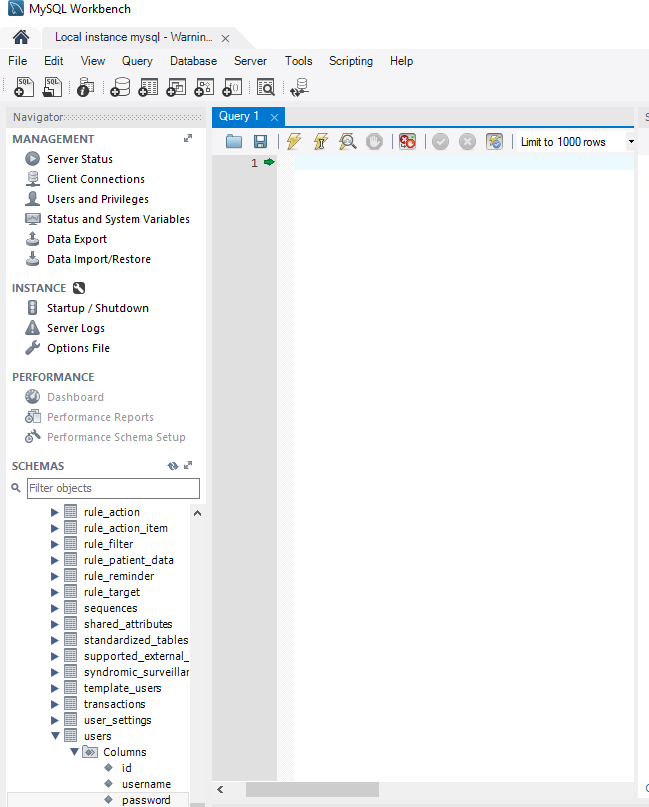
\includegraphics[width = 15cm, height=10cm]{password.jpg}
		\end{itemize}
		\item Tried to find login history under $instance/server_logs$, but it does not show any logs
		\item Tried to read datafile in detail so logged in MySQL with command shell
	\begin{itemize}
			\item Used command 'show databases' to show list of existing databases
				\begin{itemize}
			\item $http://dev.mysql.com/doc/refman/5.7/en/show-engine.html$
				\end{itemize}	
			\item Used command 'show open tables' to show usable table entries in each database
			\item Used command 'show tables in 'database name'' to show every arrays of that database
			\item Used command 'show columns in 'table name' in 'database name' to show each comlumns of database
			\begin{itemize}
				\item
				\includegraphics[width = 15cm, height=10cm]{untitled.jpg}
			\end{itemize}
	\end{itemize}
\vspace{10cm}
		\item Also used PHPmyAdmin on $localhost/openemr$
	\begin{itemize}
			\item Found user history(login/out, create new user...) on log tab
				\begin{itemize}
					\item
					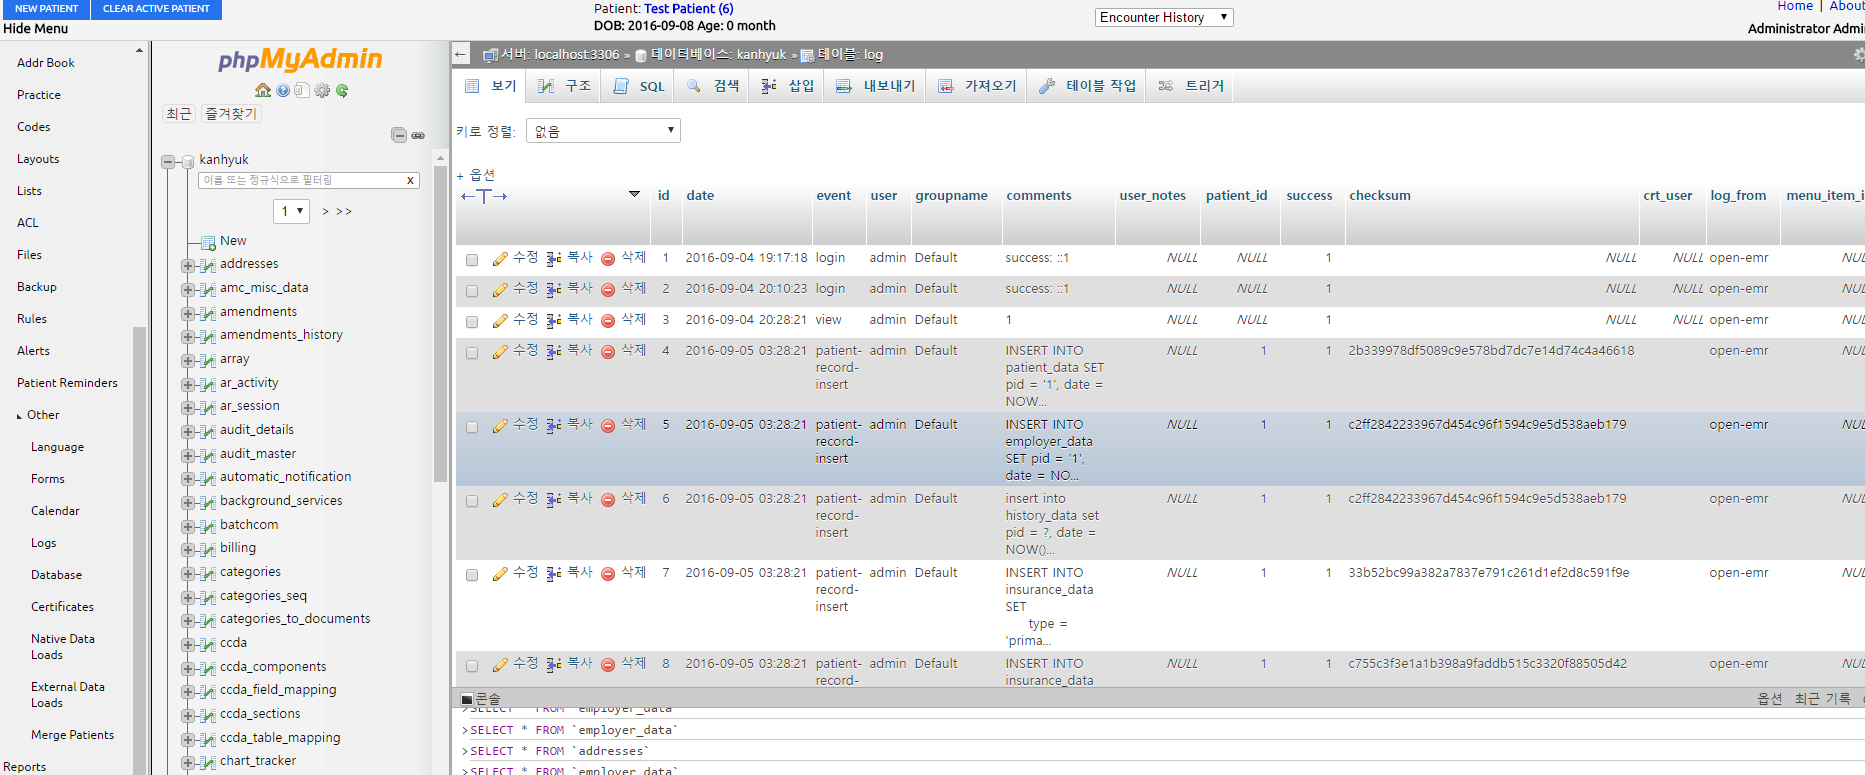
\includegraphics[width = 10cm, height=8cm]{log.jpg}
			\end{itemize}	
			\item Could find exact code when I click default values on datacolmun name
				\begin{itemize}
					\item
					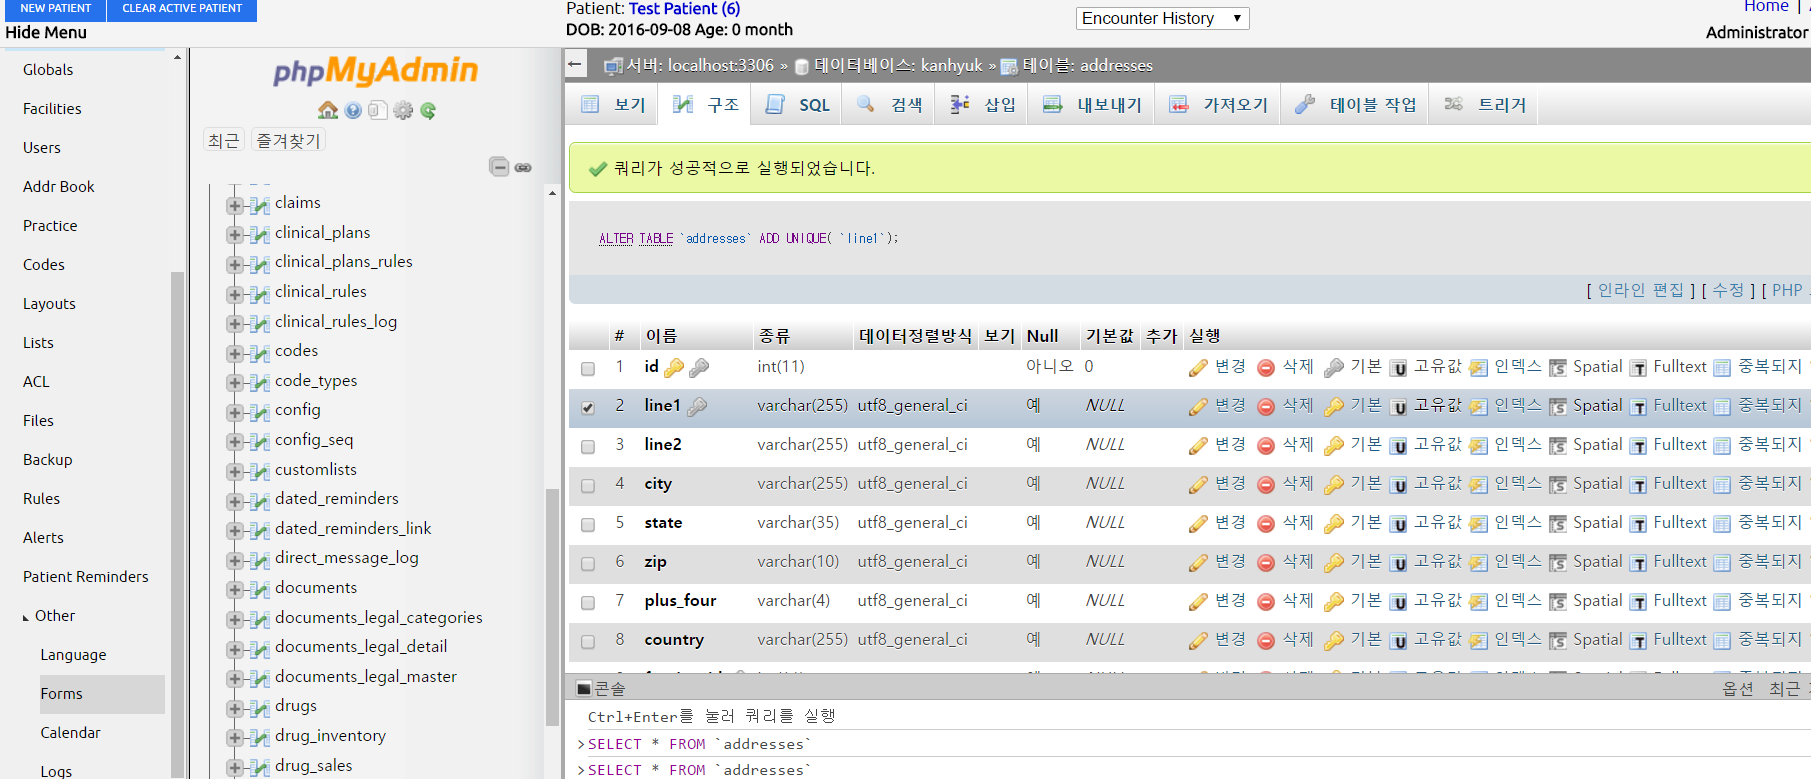
\includegraphics[width = 10cm, height=8cm]{codes.jpg}
				\end{itemize}
\vspace{5cm}
			\item We can change database name or default values on PHPmyAdmin-tablework
				\begin{itemize}
					\item
					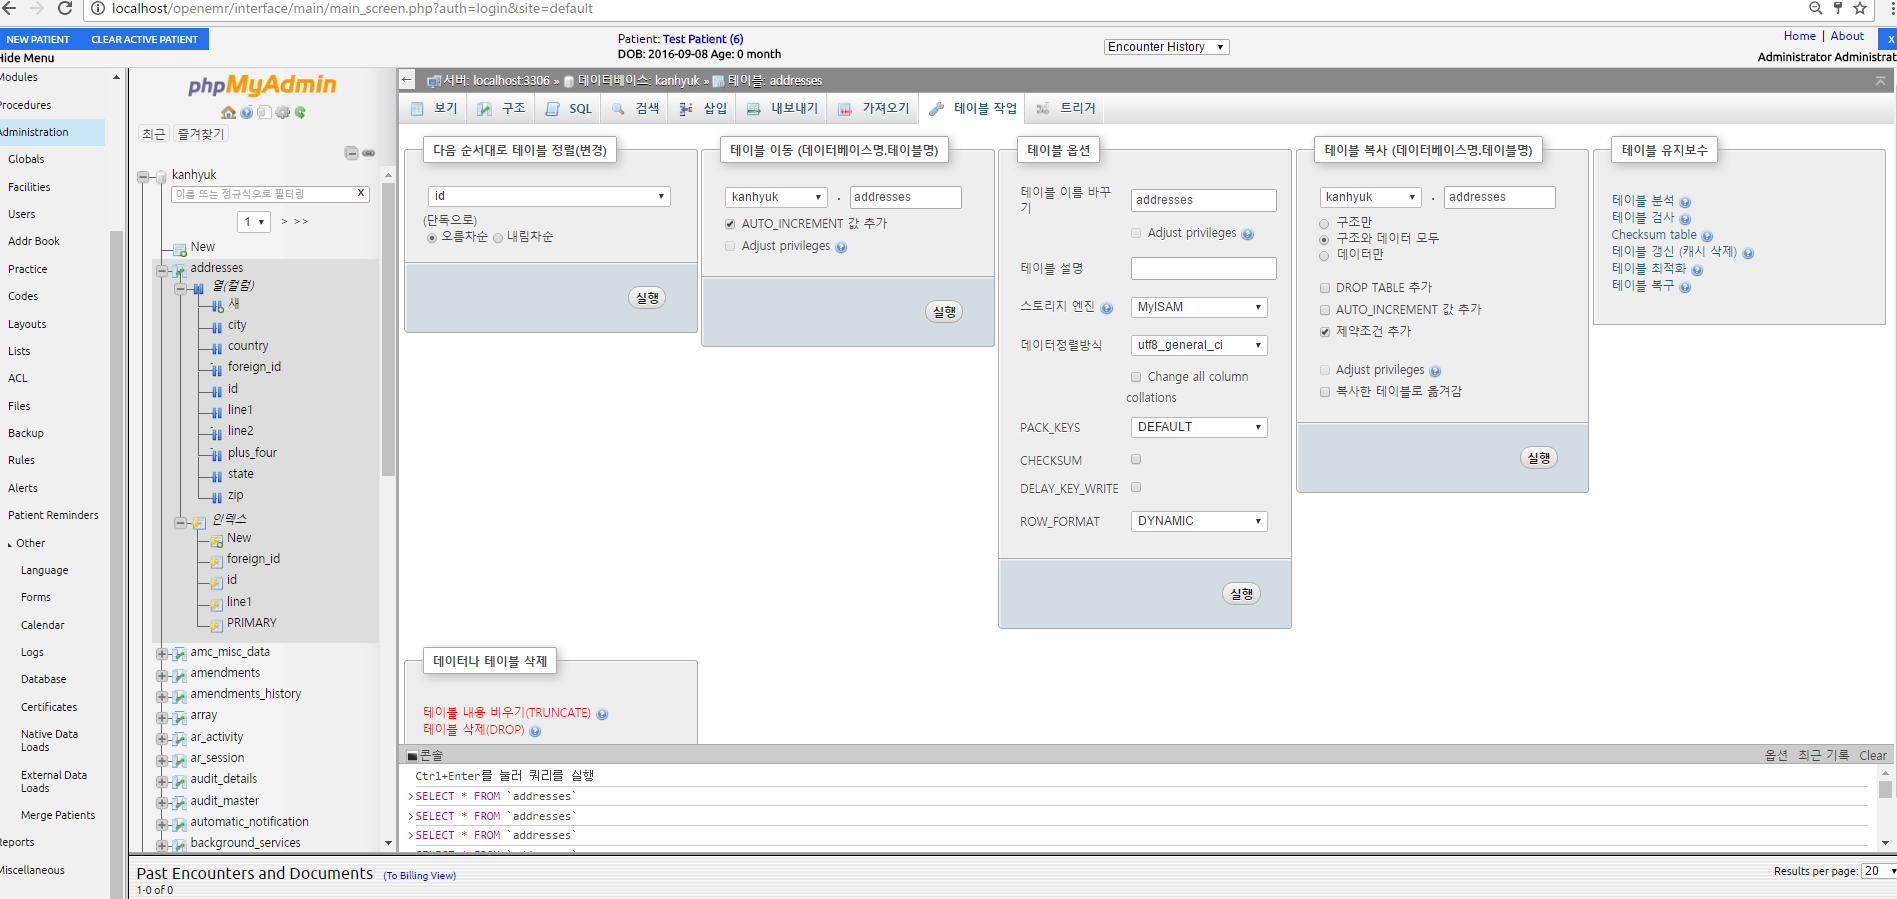
\includegraphics[width = 10cm, height=8cm]{changetables.jpg}
				\end{itemize}
			\item Amendments shows history and details(creator, created time, id)
			\item $Audit_master$ shows ipaddress, created time, id, userid
			\item Employer's data shows employer id, date, country, city
			\item $MySQLworkbench/users/columns$ shows id, username, password, autorhized...
				\begin{itemize}
					\item
					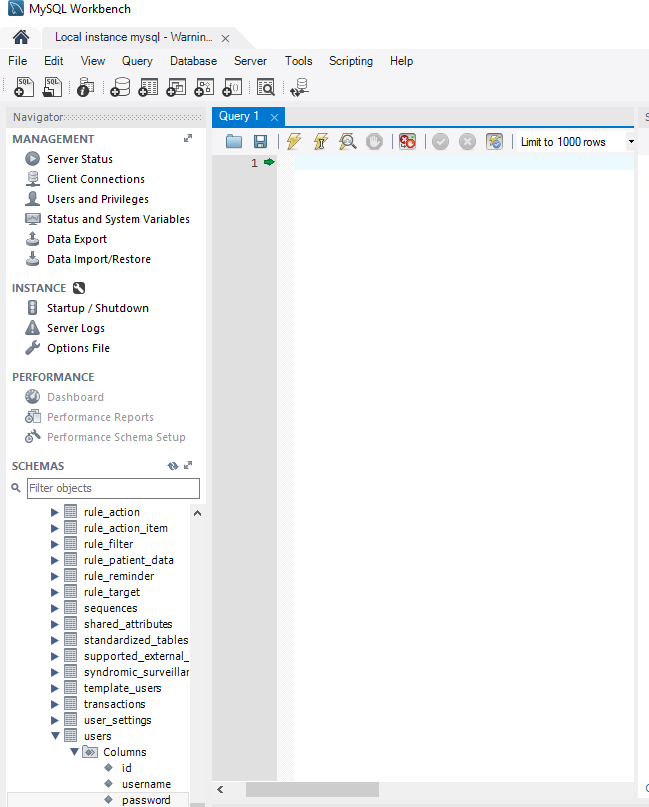
\includegraphics[width = 10cm, height=8cm]{password.jpg}
				\end{itemize}
	\end{itemize}	

\end{itemize}







\end{document}